%% For double-blind review submission
%% \documentclass[sigplan,10pt,review, anonymous]{acmart}\settopmatter{printfolios=true}
%% For single-blind review submission
%% \documentclass[sigplan,10pt,review]{acmart}\settopmatter{printfolios=true}
%% For final camera-ready submission
\documentclass[sigplan,10pt]{acmart}\settopmatter{}

%% Note: Authors migrating a paper from traditional SIGPLAN
%% proceedings format to PACMPL format should change 'sigplan,10pt' to
%% 'acmlarge'.

%% Some recommended packages.
\usepackage{booktabs}   %% For formal tables:
                        %% http://ctan.org/pkg/booktabs
\usepackage{subcaption} %% For complex figures with subfigures/subcaptions
                        %% http://ctan.org/pkg/subcaption
%% For drawing figures
\usepackage{tikz}
\usetikzlibrary{fit}

%% For typesetting code snippets
\usepackage{listings}

%% For defining syntax coloring theme
\usepackage{color}

\makeatletter\if@ACM@journal\makeatother
%% Journal information (used by PACMPL format)
%% Supplied to authors by publisher for camera-ready submission
\acmJournal{PACMPL}
\acmVolume{1}
\acmNumber{1}
\acmArticle{1}
\acmYear{2017}
\acmMonth{1}
\acmDOI{10.1145/nnnnnnn.nnnnnnn}
\startPage{1}
\else\makeatother
%% Conference information (used by SIGPLAN proceedings format)
%% Supplied to authors by publisher for camera-ready submission
\acmConference[PL'17]{ACM SIGPLAN Conference on Programming Languages}{January 01--03, 2017}{New York, NY, USA}
\acmYear{2017}
\acmISBN{978-x-xxxx-xxxx-x/YY/MM}
\acmDOI{10.1145/nnnnnnn.nnnnnnn}
\startPage{1}
\fi


%% Copyright information
%% Supplied to authors (based on authors' rights management selection;
%% see authors.acm.org) by publisher for camera-ready submission
\setcopyright{none}             %% For review submission
%\setcopyright{acmcopyright}
%\setcopyright{acmlicensed}
%\setcopyright{rightsretained}
%\copyrightyear{2017}           %% If different from \acmYear


%% Bibliography style
\bibliographystyle{ACM-Reference-Format}
%% Citation style
%% Note: author/year citations are required for papers published as an
%% issue of PACMPL.
%\citestyle{acmauthoryear}  %% For author/year citations
%\citestyle{acmnumeric}     %% For numeric citations
%\setcitestyle{nosort}      %% With 'acmnumeric', to disable automatic
                            %% sorting of references within a single citation;
                            %% e.g., \cite{Smith99,Carpenter05,Baker12}
                            %% rendered as [14,5,2] rather than [2,5,14].
%\setcitesyle{nocompress}   %% With 'acmnumeric', to disable automatic
                            %% compression of sequential references within a
                            %% single citation;
                            %% e.g., \cite{Baker12,Baker14,Baker16}
                            %% rendered as [2,3,4] rather than [2-4].

\definecolor{codegreen}{rgb}{0,0.6,0}
\definecolor{codegray}{rgb}{0.5,0.5,0.5}
\definecolor{codepurple}{rgb}{0.58,0,0.82}
\definecolor{backcolour}{rgb}{0.95,0.95,0.92}


\lstdefinestyle{snippet-theme}{
    backgroundcolor=\color{backcolour},   
    commentstyle=\color{codegreen},
    keywordstyle=\color{magenta},
    numberstyle=\tiny\color{codegray},
    stringstyle=\color{codepurple},
    % basicstyle=\,
    breakatwhitespace=false,         
    breaklines=true,                 
    captionpos=b,                    
    keepspaces=true,                 
    numbers=left,                    
    numbersep=2pt,                  
    showspaces=false,                
    showstringspaces=false,
    showtabs=false,                  
    tabsize=4
  }
  
  \lstset{style=snippet-theme}

  
  \begin{document}

%% Title information
%% [Short Title] is optional;
%% when present, will be used in
%% header instead of Full Title.
\title[Short Title]{Promises are meant to be broken}

%% \titlenote is optional;
%% can be repeated if necessary;
%% contents suppressed with 'anonymous'
%% \titlenote{with title note}             

%% \subtitle is optional
\subtitle{Strictness Analysis for R}

%% \subtitlenote is optional;
%% can be repeated if necessary;
%% contents suppressed with 'anonymous'
%%\subtitlenote{with subtitle note}     

%% Author information
%% Contents and number of authors suppressed with 'anonymous'.
%% Each author should be introduced by \author, followed by
%% \authornote (optional), \orcid (optional), \affiliation, and
%% \email.
%% An author may have multiple affiliations and/or emails; repeat the
%% appropriate command.
%% Many elements are not rendered, but should be provided for metadata
%% extraction tools.

%% Author with single affiliation.
\author{Author 1}
\authornote{with author1 note}          %% \authornote is optional;
                                        %% can be repeated if necessary
\orcid{nnnn-nnnn-nnnn-nnnn}             %% \orcid is optional
\affiliation{
  \position{Position1}
  \department{Department1}              %% \department is recommended
  \institution{Institution1}            %% \institution is required
  \streetaddress{Street1 Address1}
  \city{City1}
  \state{State1}
  \postcode{Post-Code1}
  \country{Country1}
}
\email{first1.last1@inst1.edu}          %% \email is recommended

%% Author with two affiliations and emails.
\author{Author 2}
\authornote{with author2 note}          %% \authornote is optional;
                                        %% can be repeated if necessary
\orcid{nnnn-nnnn-nnnn-nnnn}             %% \orcid is optional
\affiliation{
  \position{Position2a}
  \department{Department2a}             %% \department is recommended
  \institution{Institution2a}           %% \institution is required
  \streetaddress{Street2a Address2a}
  \city{City2a}
  \state{State2a}
  \postcode{Post-Code2a}
  \country{Country2a}
}
\email{first2.last2@inst2a.com}         %% \email is recommended
\affiliation{
  \position{Position2b}
  \department{Department2b}             %% \department is recommended
  \institution{Institution2b}           %% \institution is required
  \streetaddress{Street3b Address2b}
  \city{City2b}
  \state{State2b}
  \postcode{Post-Code2b}
  \country{Country2b}
}
\email{first2.last2@inst2b.org}         %% \email is recommended


%% Paper note
%% The \thanks command may be used to create a "paper note" ---
%% similar to a title note or an author note, but not explicitly
%% associated with a particular element.  It will appear immediately
%% above the permission/copyright statement.
\thanks{with paper note}                %% \thanks is optional
                                        %% can be repeated if necesary
                                        %% contents suppressed with 'anonymous'


%% Abstract
%% Note: \begin{abstract}...\end{abstract} environment must come
%% before \maketitle command
\begin{abstract}
R evaluates function arguments lazily. When a function is called the formal
parameters are bound to ``promises'' Arguments are stored in ``promises''
which are ``forced'' when the corresponding parameter is used in an evaluation context. A
promise also contains a reference to the environment in which the argument has
to be evaluated and a slot to cache the result of evaluation.  This mechanism
can potentially improve speed of R programs by preventing the evaluation of
arguments that are not used. However, benchmarks obtained by instrumenting the R
interpreter indicate that lazy evaluation is futile for majority of R programs
and detrimental for their performance. R has a functional core and even most the
basic control structures are implemented as functions. This results in the
creation of a huge number of promises which get forced immediately but continue
storing the unevaluated arguments until they are garbage collected. Furthermore,
accessing the argument's value requires the promise to look up the cache which
introduces a level of indirection, increasing the possibility of cache misses.

%% TODO - Why is evaluation order important?

In this paper, we present a static analysis technique on an intermediate
representation of R code that identifies the promises that are forced and the
order in which they are forced. This information can then be used by an
optimizer to prevent the creation of promises and evaluate arguments in the
correct order, ensuring unchanged program behavior. We validate the results of
our static analysis from dynamic runs on a number of widely used R libraries.
\end{abstract}

%% 2012 ACM Computing Classification System (CSS) concepts
%% Generate at 'http://dl.acm.org/ccs/ccs.cfm'.
\begin{CCSXML}
<ccs2012>
<concept>
<concept_id>10003752.10010124.10010138.10010143</concept_id>
<concept_desc>Theory of computation~Program analysis</concept_desc>
<concept_significance>500</concept_significance>
</concept>
<concept>
<concept_id>10011007.10011006.10011008.10011024.10011035</concept_id>
<concept_desc>Software and its engineering~Procedures, functions and subroutines</concept_desc>
<concept_significance>300</concept_significance>
</concept>
<concept>
<concept_id>10011007.10011006.10011008.10011009.10011021</concept_id>
<concept_desc>Software and its engineering~Multiparadigm languages</concept_desc>
<concept_significance>100</concept_significance>
</concept>
</ccs2012>
\end{CCSXML}
\ccsdesc[500]{Theory of computation~Program analysis}
\ccsdesc[300]{Software and its engineering~Procedures, functions and subroutines}
\ccsdesc[100]{Software and its engineering~Multiparadigm languages}
%% End of generated code

%% Keywords
%% comma separated list
%% \keywords is optional
\keywords{R, Strictness analysis, Control-Flow analysis,
  Static analysis, Program analysis, Performance optimization}

%% \maketitle
%% Note: \maketitle command must come after title commands, author
%% commands, abstract environment, Computing Classification System
%% environment and commands, and keywords command.
\maketitle

\section{Introduction}

Text of paper \ldots

\section{Overview}

\subsection{Promise}

A promise object has three slots; value, expression and environment. When a
function is called, the actual arguments are wrapped inside promises. The
promise also contains a reference to the 


\begin{figure}
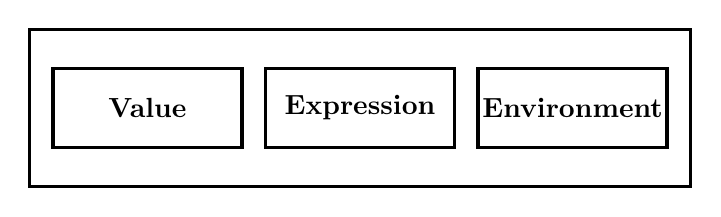
\begin{tikzpicture}[font=\sffamily\small]
  \begin{scope}%[blend group = soft light]
    % \draw[help lines] (-4,1) grid (4,3);

    % \draw[fill = pink, fill opacity = 0.3,
    % draw = pink
    % , draw opacity = 1.0, very thick]
    % (-4, 1) rectangle (4, 3)
    % node[midway, pink, font=\bf] {Value};

    % \draw[fill = red, fill opacity = 0.3,
    % draw = red, draw opacity = 1.0, very thick]
    % (-3.5, 1.5) rectangle (-1.5, 2.5)
    % node[midway, red, font=\bf] {Value};

    % \draw [fill = {rgb:red,166;green,206;blue,227}, fill opacity = 0.5,
    % draw = {rgb:red,166;green,206;blue,227}, draw opacity = 1.0, very thick]
    % (-1.0, 1.5) rectangle (1.0, 2.5) node[midway, blue, font=\bf] {Expression};

    % \draw [fill = green, fill opacity = 0.3,
    % draw = green, draw opacity = 1.0, very thick]
    % (1.5, 1.5) rectangle (3.5, 2.5) node[midway, green, font=\bf] {Expression};
    
    % \draw [fill = red!10, ultra thick, red!60] (-1.0, -1) rectangle ( 1.0, 1);
    % \draw [fill = red!10, ultra thick, red!60] ( 1.5, -1) rectangle ( 3.5, 1);
    \draw[very thick](-4.2, 0.0) rectangle ( 4.2, 2.0); % node[anchor=north, font=\bf] {Promise};
    \draw[very thick](-3.9, 0.5) rectangle (-1.5, 1.5) node[midway, font=\bf] {Value};
    \draw[very thick](-1.2, 0.5) rectangle ( 1.2, 1.5) node[midway, font=\bf] {Expression};
    \draw[very thick]( 1.5, 0.5) rectangle ( 3.9, 1.5) node[midway, font=\bf] {Environment};
    
  \end{scope}
\end{tikzpicture}
\caption{Structure of a promise.} %\label{fig:Structure of a promise}
\end{figure}

\subsection{Background on R/Strictness}



\subsection{Example/IR representation}

\lstinputlisting[language=R]{side-effect.R}
% \begin{lstlisting}[language=R]
% \end{lstlisting}
% TODO - Informal discussion of analysis
\section{Algorithm}

\section{Implementation}
% TODO - Discuss implementation and other pragmatic issues.

\section{Experimental Results}
\begin{itemize}
\item Percentage of promises evaluated in the first arguments.
\item Percentage of promises with side effects.
\item Percentage of promises never evaluated.
\item Percentage of promises escaping to other functions and being evaluated.
\item Promises which are evaluated in different order in different tests.
\item Compare this with the result of strictness analysis.
\end{itemize}
% TODO - Discuss research problems, experimental setup, experiments and draw
% conclusion on these experiments.

\section{Related Work}

\section{Conclusions}

%% Acknowledgments
\begin{acks}                            %% acks environment is optional
                                        %% contents suppressed with 'anonymous'
  %% Commands \grantsponsor{<sponsorID>}{<name>}{<url>} and
  %% \grantnum[<url>]{<sponsorID>}{<number>} should be used to
  %% acknowledge financial support and will be used by metadata
  %% extraction tools.
  This material is based upon work supported by the
  \grantsponsor{GS100000001}{National Science
    Foundation}{http://dx.doi.org/10.13039/100000001} under Grant
  No.~\grantnum{GS100000001}{nnnnnnn} and Grant
  No.~\grantnum{GS100000001}{mmmmmmm}.  Any opinions, findings, and
  conclusions or recommendations expressed in this material are those
  of the author and do not necessarily reflect the views of the
  National Science Foundation.
\end{acks}


%% Bibliography
\bibliography{references}


%% Appendix
\appendix


\section{Appendix}

Text of appendix \ldots

\end{document}